\section{\label{I-B-2}Conséquences. Le cas de la migration vers la plateforme de \gls{clade}}

Lors des missions qui ont été réalisées durant ce stage, cette contrainte s'est surtout manifestée dans les outils informatiques de catalogage et de diffusion des collections imposé au \mae. Les chantiers de mise en place de nouveaux logiciels qui se sont achevé cet été 2025 ont par exemple tous deux été pilotés par le \minarm : la mise en place du logiciel de gestion des collections \gls{archange} (\textit{S-Museum} de \textit{Skinsoft}) s'inclut dans un projet progressif d'intégration des musées du ministère sur une même plateforme de gestion des collections. La migration vers le \ac{sigb} \gls{koha} pour la bibliothèque, et la diffusion de ses collections sur la plateforme \gls{clade} s'inscrit dans un projet similaire pour toutes les bibliothèques du ministère, afin d'unifier leur gestion mais aussi d'améliorer leur accessibilité en permettant à l'utilisateur d'interroger sur le même portail l'ensemble des \gls{bibmusee}.

Le musée peut ainsi se retrouver dans des positions délicates : dans le cas de la migration vers \gls{clade}, à laquelle j'ai pu être confrontée lors de mon stage, les responsables du \ac{drd} ont du faire face à des difficultés particulières, directement causées par l'intégration de la bibliothèque du \mae à un réseau qui lui est plus large. D'un côté en effet, ce projet offre de grands avantages en matière d'accessibilité des catalogues : centralisation de la recherche, recherche par mots-clés, intégration de documents numériques téléchargeables par exemple\footcite{ministeredesarmeesKitCommunicationCLADE}. Elle permet aussi à des institutions plus petites de participer à un projet qu'elles n'auraient peut-être pas eu les ressources de mener indépendamment. Cependant, cela signifie également qu'il devient plus délicat de s'adapter aux exigences et aux habitudes de gestion de chacun, ce qui devient problématique dans le cas de bibliothèques spécialisées comme celle du \mae. Par exemple, le projet est géré à l'échelle du ministère : cela signifie que pendant toute sa durée, les agents du \ac{drd} n'ont eu que très peu de visibilité sur le déroulé de la migration : ceux-ci n'ont par exemple jamais eu accès à au cahier des charges du projet. Il devient donc difficile pour les utilisateurs d'identifier d'éventuels problèmes pendant la migration : ce n'est qu'à la fin de la phase de test qu'il a été découvert que la structure du fichier d'import du thésaurus avait été mal comprise par les chargés de la migration des données, et que ceci avait causé des inexactitudes lors de l'import, extrêmement difficiles à corriger après coup.

Au-delà des problèmes d'import, la configuration même d'une telle plateforme représente de réels défis, qui ne sont pas encore pleinement résolus : comme le manifestent les captures d'écran de l'interface web ci-dessous\footnote{Voir la figure \ref{fig:clade_histoaviation}}, \gls{clade} offre une interface moderne et ergonomique. Celle-ci permet d'effectuer des recherches par mot-clé et par institution (appelées \enquote{portails}). Des filtres permettent de préciser la recherche et chaque utilisateur peut se constituer un panier, sauvegarder des favoris\dots autant de fonctionnalités qui n'existaient pas de manière aussi avancées dans l'ancien logiciel \gls{alexandrie}. Un nuage de mots-clés permet même d'avoir un aperçu rapide des connaissances englobées par la recherche de l'utilisateur. En se penchant sur les notices, le défi représenté par ce regroupement -- et les exigences d'interopérabilité qui en découlent pour le \mae -- devient manifeste : chaque institution ayant ses habitudes de catalogage propres, réconcilier les différents ouvrages devient difficile lorsque la mise en forme du contenu des champs, les champs eux-mêmes et la structuration du thésaurus diffèrent d'un même ouvrage à l'autre selon le producteur de la notice.


\begin{figure}[htbp]
	\centering
	\begin{subfigure}{0.7\textwidth}
		\centering
		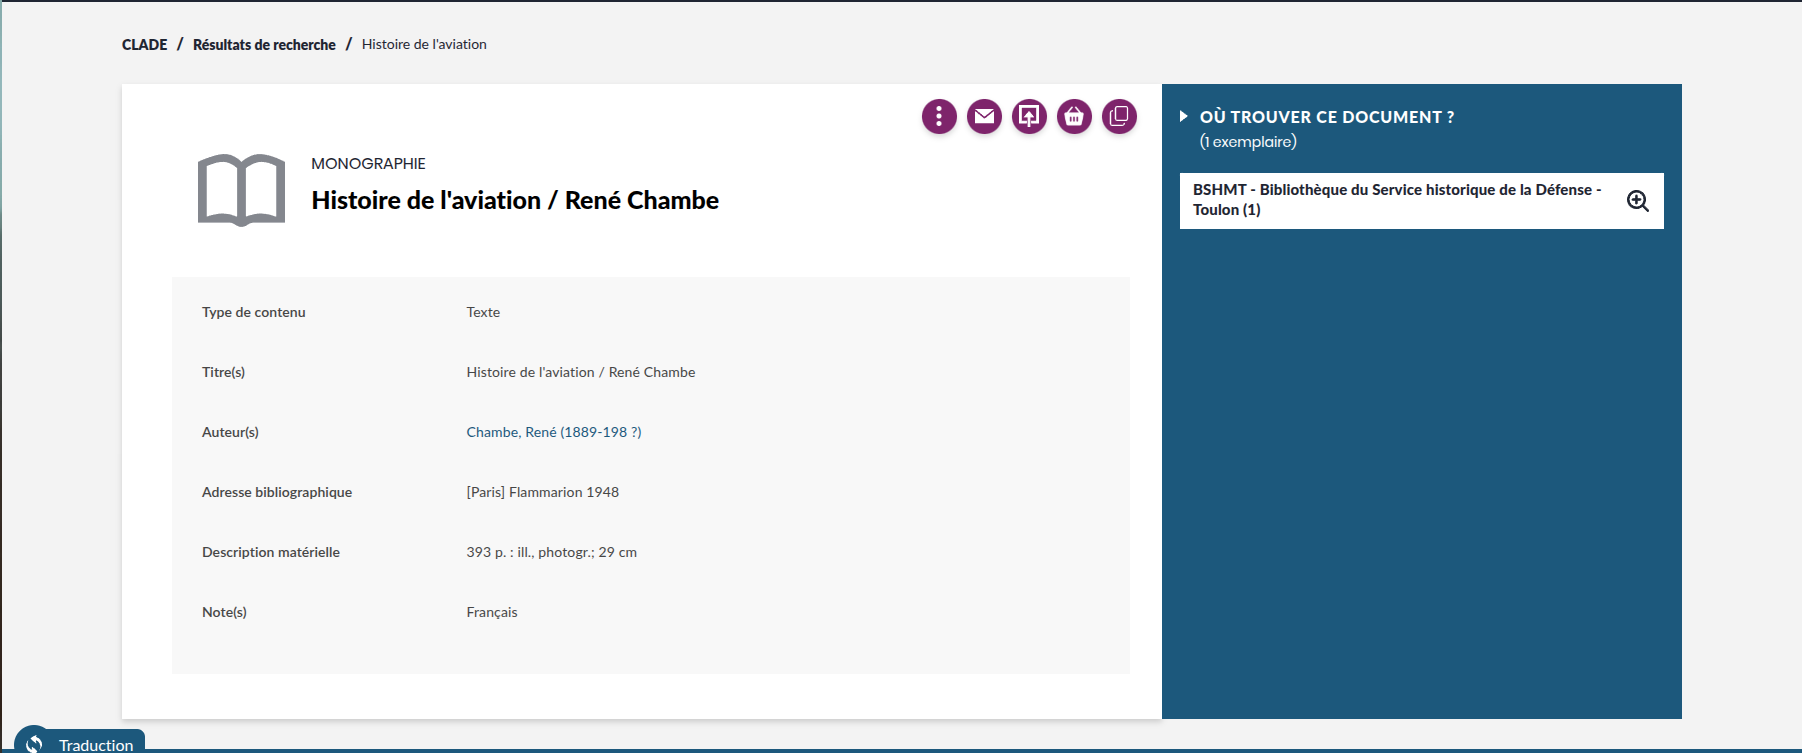
\includegraphics[width=\linewidth]{img/IMG_clade_histoireaviation_shdTL}
		\caption{Service Historique de la Défense}
		\label{img:cladehistoireaviationshdtl}
	\end{subfigure}
	\begin{subfigure}{0.7\textwidth}
		\centering
		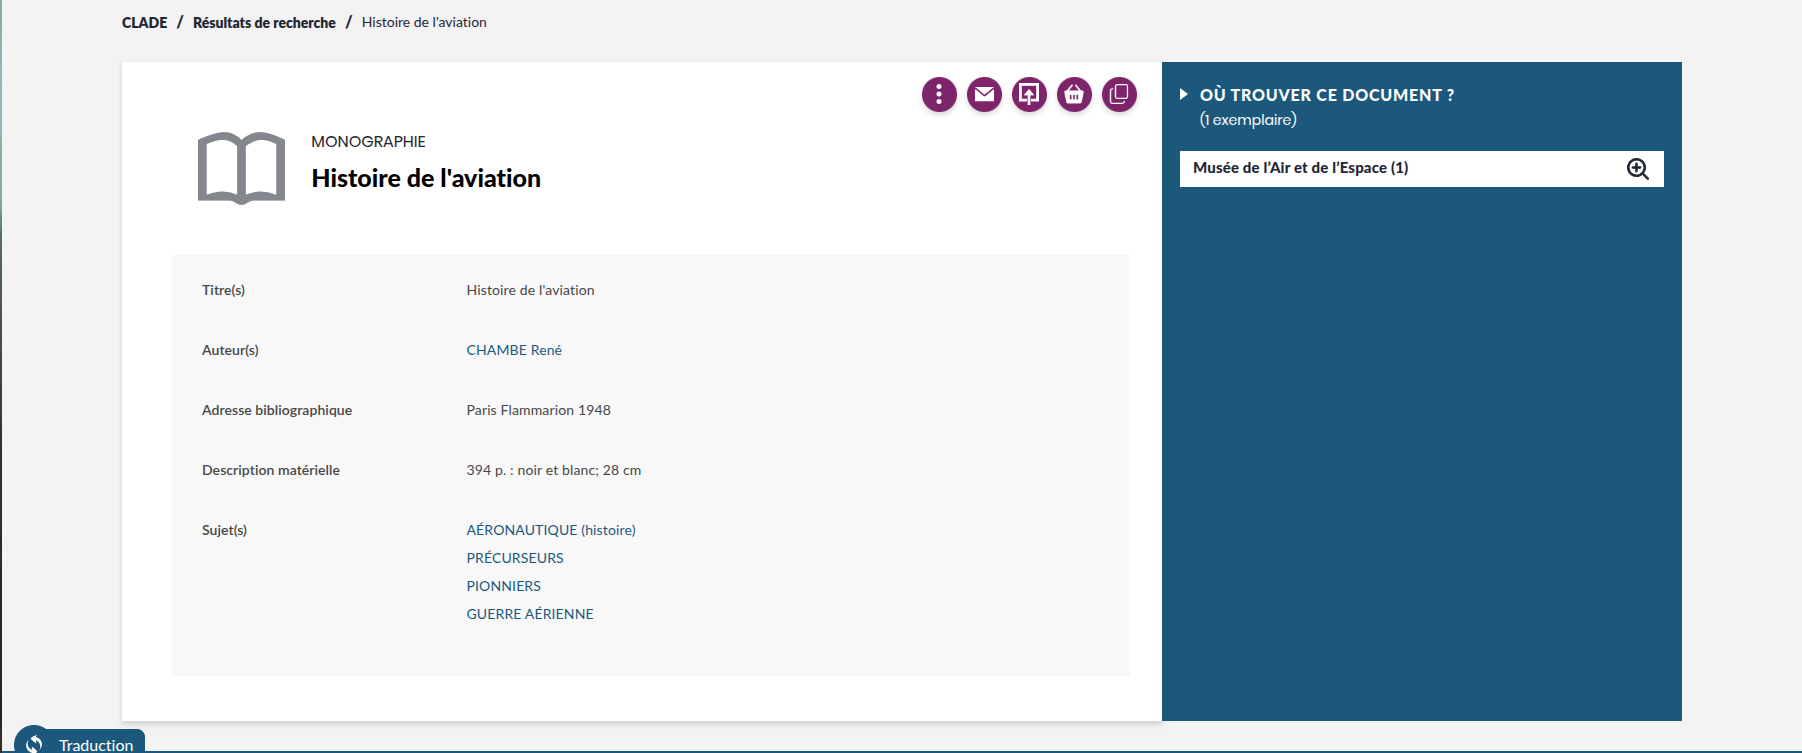
\includegraphics[width=\linewidth]{img/IMG_clade_histoireaviation_mae}
		\caption{\mae}
		\label{img:cladehistoireaviationsmae}
	\end{subfigure}
	\hfill
	\begin{subfigure}{0.7\textwidth}
		\centering
		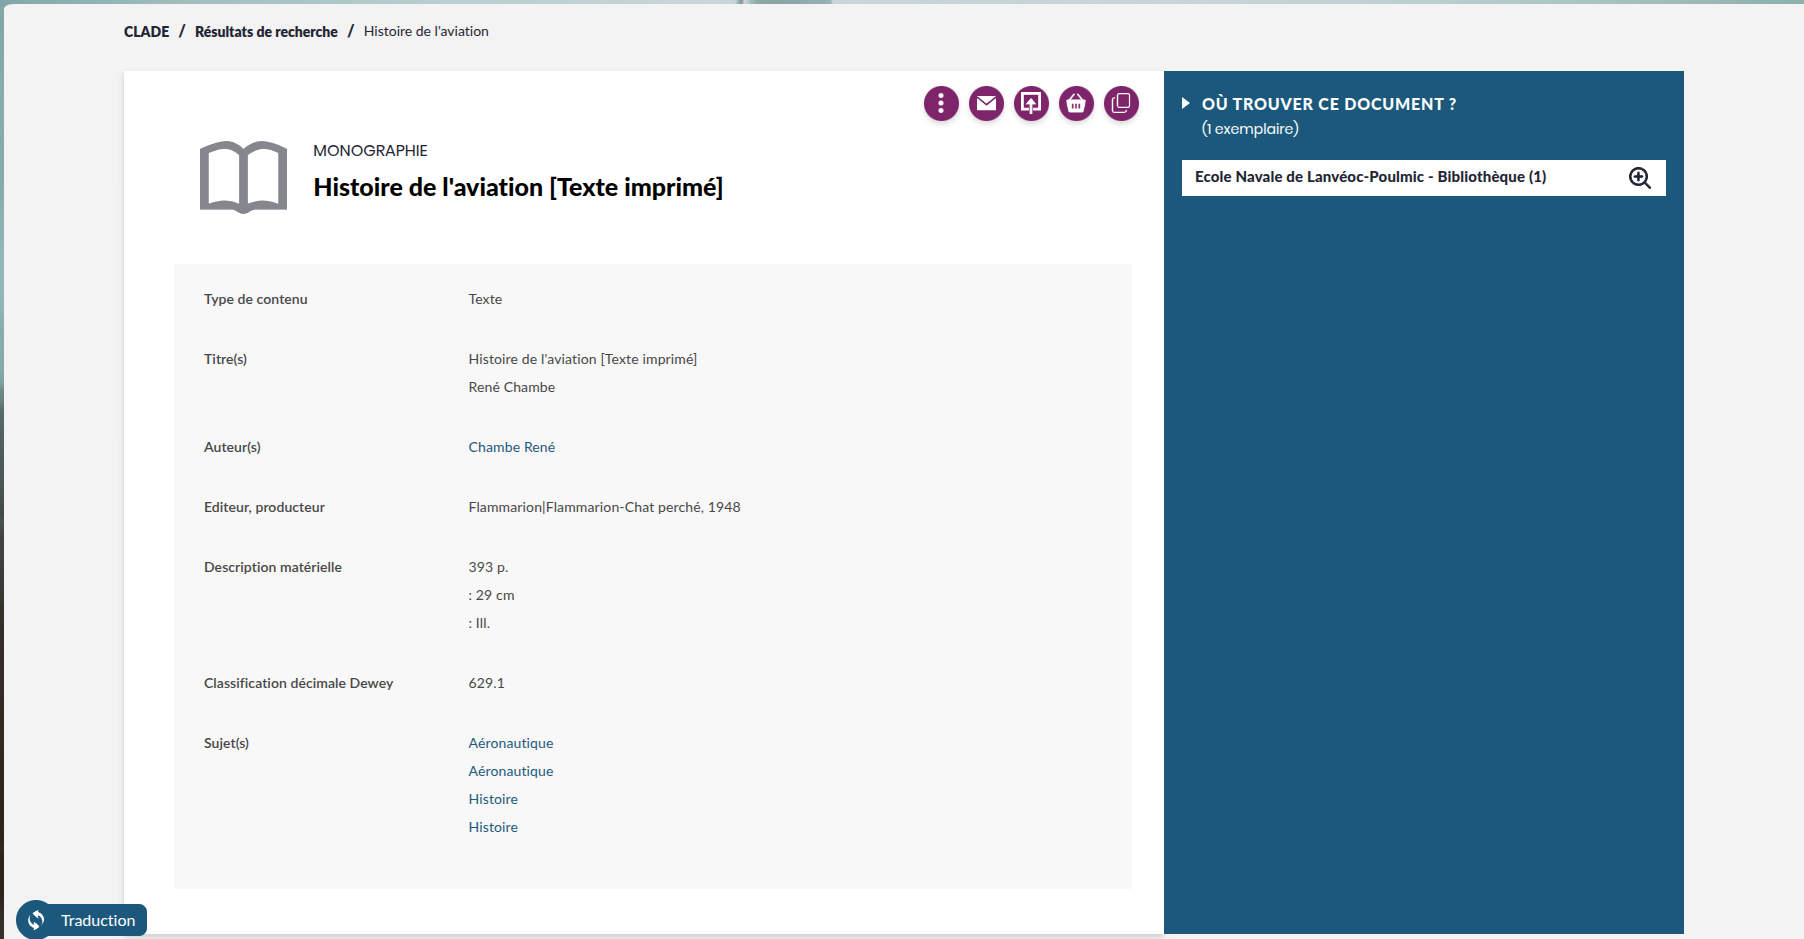
\includegraphics[width=\linewidth]{img/IMG_clade_histoireaviation_navale}
		\caption{École navale}
		\label{img:cladehistoireaviationnavale}
	\end{subfigure}
	\caption[Différences de catalogage entre les \bibmusee sur \ac{clade}]{Malgré la volonté de mise en commun sur \ac{clade}, la même édition d'un même ouvrage peut être cataloguée de plusieurs manières différentes et apparaître comme des ouvrages distincts : ici, l'\textit{Histoire de l'aviation} de René Chambe chez Flammarion (1948)}
	\label{fig:clade_histoaviation}
\end{figure}


La migration vers \gls{clade} illustre les tensions qui peuvent exister entre les ambitions fédératrices du \minarm et les exigences propres du \mae : chaque gain en mutualisation se paie d’une vigilance accrue pour préserver l’identité et la valeur scientifique des collections.
